\documentclass[11pt,a4paper]{jarticle}
\usepackage[dvips]{graphicx}
\usepackage{here}

\title{{チーム研究\\実験計画、サーベイ報告}}
\date{2014年5月9日(金)}
\author{小森谷 大介、川畑 裕也、深津 佳智}

\begin{document}

\maketitle

%1
\section{概要}
今年度、触入班では、以下の2つの方針を考えている。
\begin{itemize}
	\item 昨年度の研究から得た知見を基に、背面に突起もしくはくぼみを付けた新たなケースのデザインを考える。
	\item ``携帯情報端末''、``触覚''、``入力''をキーワードとして、昨年度の研究の発展案を考える。
\end{itemize}
本進捗資料においては、後者の発展案を述べる。
具体的には、スマートフォンの表面(タッチパネル)に突起を付けることにより、ユーザがタッチパネルにタッチする際の手がかりとするという発展案を考えた。
作成したプロトタイプ、及び、実験計画について報告する。

%2
\section{プロトタイプ}


%作ったプロトタイプ(ビーズを付けたフィルム)の写真を載せるといいと思う!
\begin{figure}[H]
\begin{minipage}{0.5\hsize}
  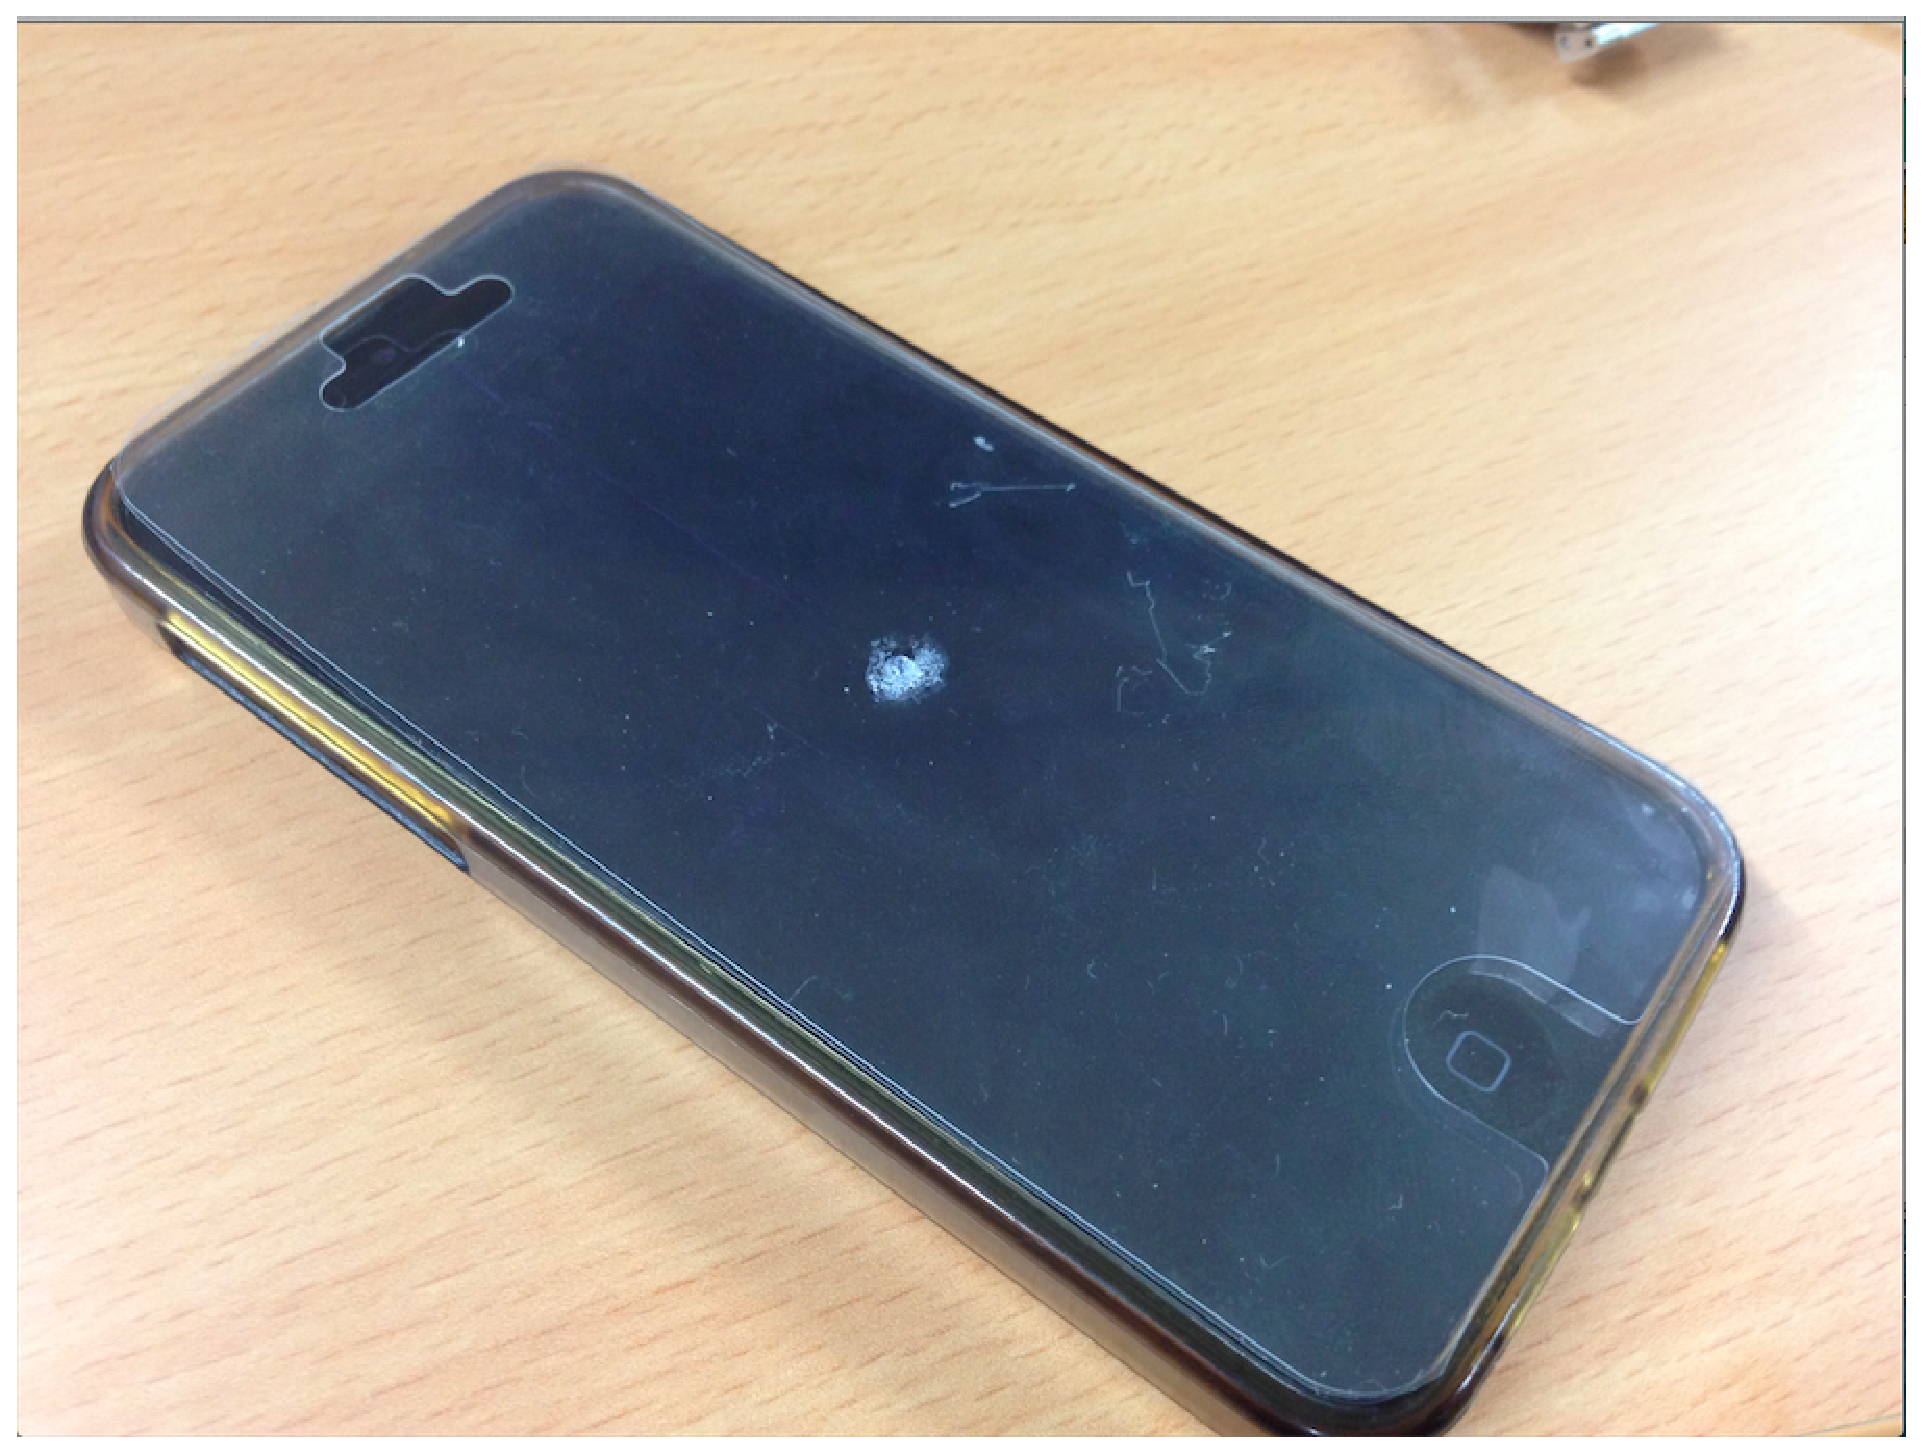
\includegraphics[width=3cm]{fig/figure4.eps}
  \caption{フィルムA}
\end{minipage}
%\end{figure}
%\begin{figure}
\begin{minipage}{0.5\hsize}
  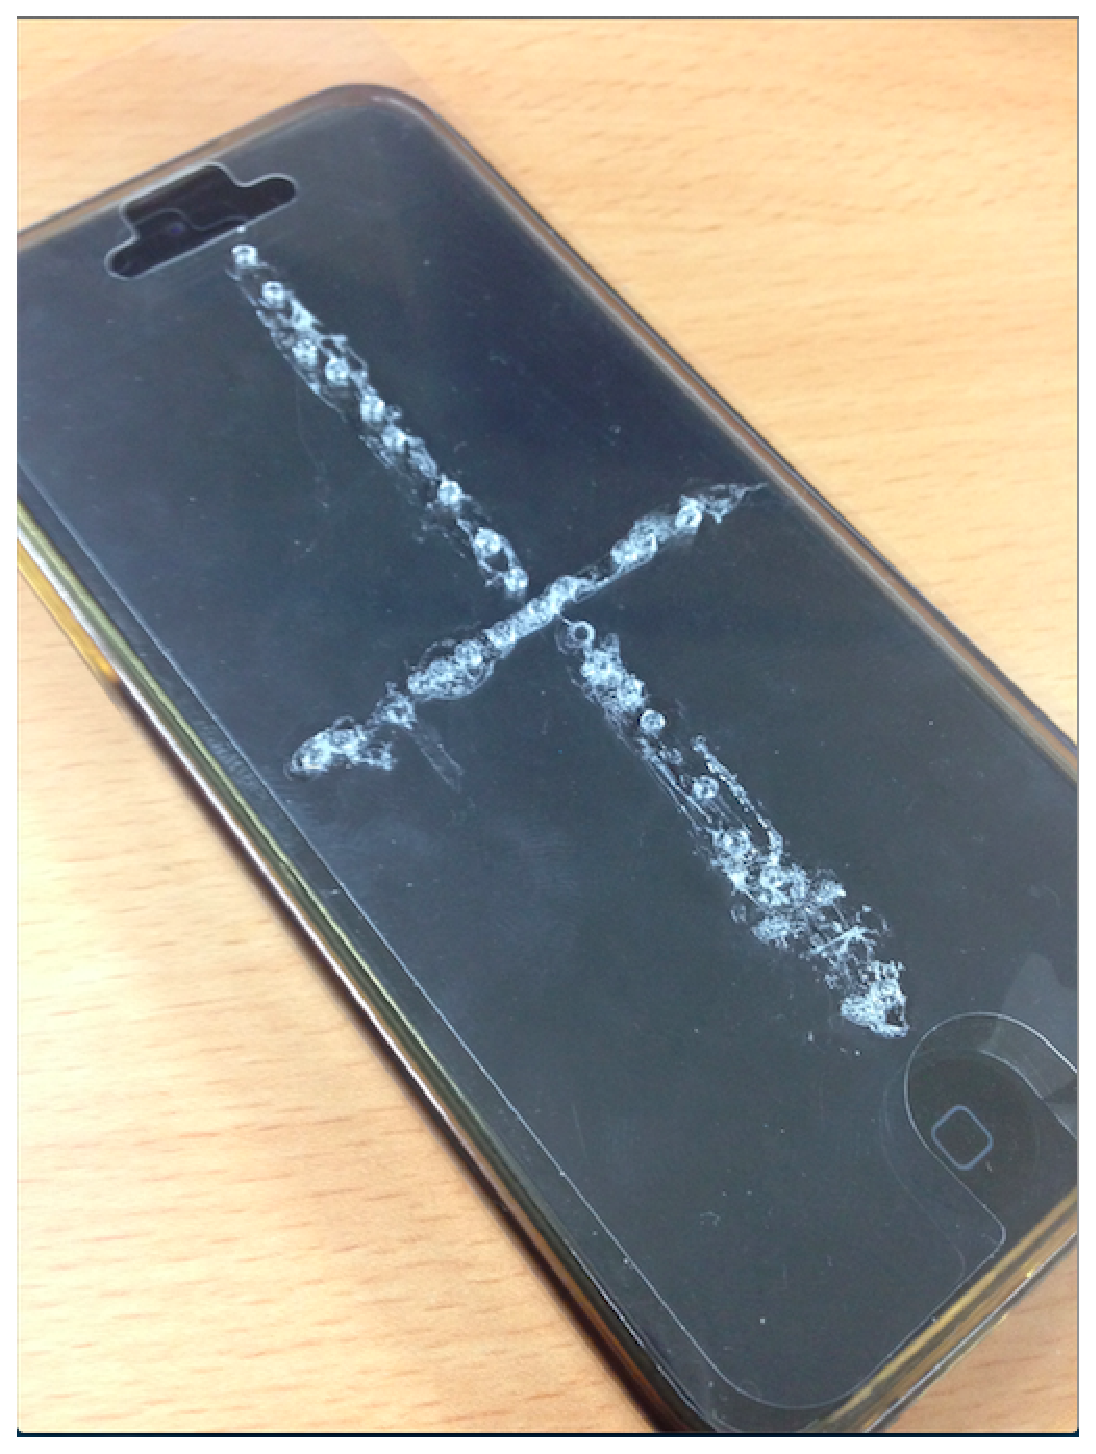
\includegraphics[width=3cm]{fig/figure5.eps}
  \caption{フィルムB}
\end{minipage}
\end{figure}

%3
\section{実験計画}
作成したプロトタイプを用いて、昨年度のソフトウェア科学会大会投稿時の実験と同様の実験を行うことを考えている。
具体的には、
\begin{itemize}
	\item フィルム条件:フィルム無し条件、フィルムA条件、フィルムB条件
	\item タッチ条件:開始点タッチ条件、終了点タッチ条件
	\item 分割条件:3~$\times$~3分割条件、4~$\times$~4分割条件、5~$\times$~5分割条件
\end{itemize}
の3種類の実験条件を設定し、被験者にアイズフリーにおいてタッチパネル上のターゲットをタッチしてもらう実験を行うことを考えている。
昨年度の実験と今回の実験計画の相違点は、ケース条件であったところをフィルム条件に変えた点である。
表面に付いている突起をタッチの手がかりとできるので、特に、終了点タッチ条件の際のタッチ精度向上が望める(昨年度の実験では、開始点タッチ条件と終了点タッチ条件のタッチ精度に有意差は見られなかった)。

%4
\section{サーベイ}
主に、タッチパネルの表面に工夫を施した研究をサーベイした。
これらのサーベイを報告する。

%4.1
\subsection{I Feel it in my Fingers: Haptic Guidance on Touch Surfaces\cite{Zimmermann:2014}}
\subsubsection{概要}
運転中に視覚を用いない操作を行うために、4つのシリコン箔をタブレットデバイスの表面に貼り付け触覚ガイダンスとし、車載アプリケーションのプロトタイプを作成した。


\subsubsection{実験機器}
触覚ガイダンスとして、初期のプロトタイプにおいては紙を使用したがタッチを感知することができなかったため、シリコン箔を使用することとした。シリコン箔(厚さ0.5mm)を真空吸着とテープの2つを用いてタブレットの表面に貼付けた。シリコン箔には縁をホイルを用いて覆ったものとそうでないものの2種類を作成した。
実験にはAndroidを搭載したAsus製のEee Padを使用した。
シリコン箔は伝統的にボタンが配置されている位置と、ユーザが任意に決めた位置の2種類の配置を行った。

\subsubsection{実験}
評価には2種類のシリコン箔の配置とタッチ方法と縁のあるなし、そして2種類の触り方についてのテストを行った。被験者は20歳から40歳の12人の学生と博士とした。

実験のタスクは各手法のシンボルをランダムな順序に並べた16個のシンボルを選ぶことである。全ての被験者は実行例を含む導入フェーズのあと実験に入った。それぞれのシンボルについて正解がタッチできたかを音声によって発表し、正解した場合は3秒後に次のシンボルへ移行した。

\subsubsection{結果}
すべての参加者が触覚からボタンを発見し、画面を見ることなく操作を行うことができた。シリコン箔の縁についても明確に区別をできた。

ユーザが任意に決めた位置にシリコン箔を置くことはボタンの位置に固定することよりもエラーが少なく、視線を向けることが少ないことがわかった。被験者の手のサイズに合わせてシリコン箔を設置することができることは被験者は好きであった。

被験者のアンケートと実行時間からユーザが任意に決めた位置にシリコン箔を設置しドラックすることがもっとも良い評価と実行時間を得られることがわかった。

\begin{figure}[H]
  \begin{center}
  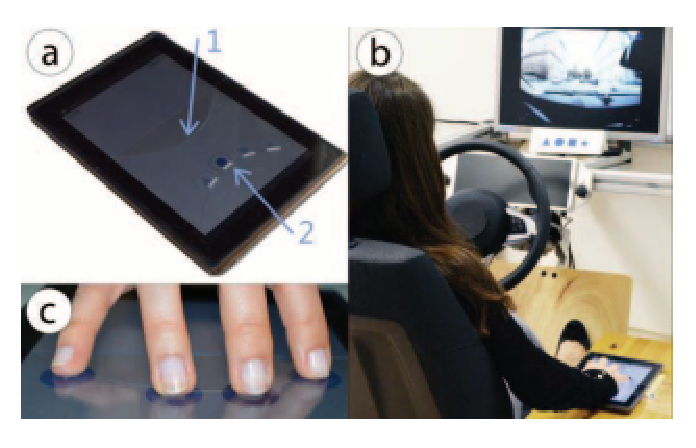
\includegraphics[width=8cm]{fig/figure1.eps}
  \caption{a:シリコン箔を貼り付けたタブレットb:実験の様子c:ユーザがボタンを任意の位置に決めた状態}
  \label{fig:1_test}
  \end{center}
\end{figure}


%4.2
\subsection{BackTap: robust four-point tapping on the back of an off-the-shelf smartphone\cite{Zhang:2013}}
\subsubsection{概要}
スマートフォンの背面ケースに4つの異なるタッチパネルを追加する入力方式を提示する。これにより歩きながら、または画面を押さえながら目を向けることなくスマートフォンの操作をすることが出来る。
本手法においてはスマートフォンに組み込まれたマイク、ジャイロスコープ、加速度計の3つのセンサを使用して軽い実装を実現した。

\subsubsection{実装と考察}
スマートフォンの3つの組み込みのセンサから得られたデータを組み合わせて背面のタップを検知することとした。初期においては加速度のみを使用していたが試行錯誤の末に3つのデータをすべて使用しなければタップを検知できないことがわかった。また、モーションごとにパラメータの変更が必要なことがわかったため機械学習の使用も考慮したいと考えている。

%4.3
\subsection{Tactile Rendering of 3D Features on Touch Surfaces\cite{Kim:2013}}
\subsubsection{概要}
タッチスクリーンに幾何学的な特徴をシュミレートするための触覚レンダリングを示す。これは、物理的に動かすのではなく、ユーザの指とタッチスクリーンの間の摩擦を調整することによってシュミレートを行う。

\subsubsection{摩擦フィードバック}
摩擦の知覚モデルとしてディスプレイに加圧される電圧の関数を定式化する。摩擦の知覚レベルを調節し、複雑な3Dオブジェクトのための触覚フィードバックを行うためにこのモデルを利用する。触覚フィードバックについては先行研究に基づく。

\subsubsection{実験}
先行研究の触覚の一般的な制御方式と今回の摩擦レンダリングの手法との比較実験を行う。パネル上に電圧の周波数と振幅を検知するトランジスタの回路と静電容量パネルを取り付けて構成された実験機を用いる。

実験は6人の男性を被験者とし、被験者は人差し指でタッチパネルをなぞり、自由に動かした。その後主観的な摩擦強度を0から100までの番号を割り当てた。

被験者には10Hzずつに等間隔に110~220Hzの摩擦レベルをランダムに30回出現させた。実験前に被験者は評価尺度と導入の説明を受け、環境とデバイスのノイズを遮断するためイヤーマフを身につけた。

\subsubsection{結果}
結果を分析したところ、周波数は結果に明確な関係はなく、フィードバックを行う幅と高さの分散が有意であることがわかった。


\begin{figure}[H]
  \begin{center}
  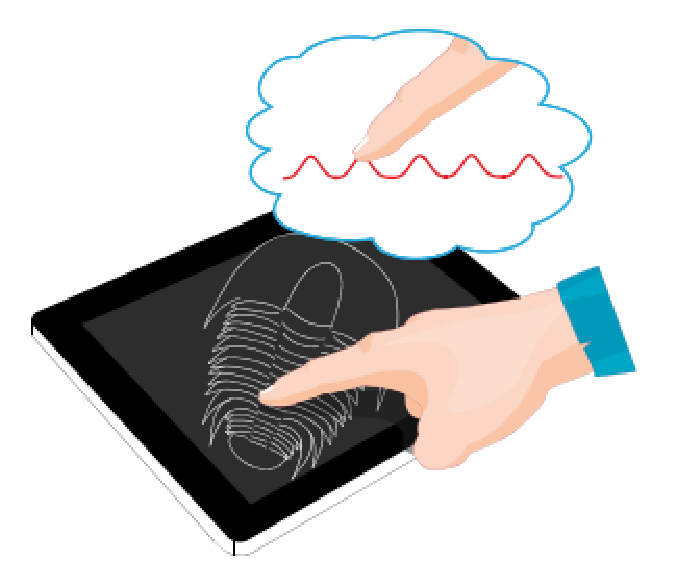
\includegraphics[width=8cm]{fig/figure2.eps}
  \caption{摩擦フィードバックのイメージ図}
  \label{fig:1_test}
  \end{center}
\end{figure}

%4.4
\subsection{Tactile Guides for Touch Screen Controls\cite{Kincaid:2012:TGT:2377916.2377963}}
\subsubsection{概要}
タブレット端末に透明のガイドを乗せることにより触覚を提示する。このガイドはボタン、スライダ及びノブの形に切り抜かれている。

\subsubsection{実験}
ノブを二つ使用する。一つはx軸、一つはy軸を操作するものである。被験者はこの二つのノブを用いて画面上にある点を移動させる。被験者が点をターゲットまで移動させる時間を測定する。これを透明のガイドあり、なしの両方において測定し、時間を比較した。


\subsubsection{結果と考察}
結果はガイドありのほうが優位に早かった。ガイドを使用することによりボタン、スライダ及びノブの外形を判別することができるため素早く操作できる。
またタブレット上において触覚フィードバックを付加する類似の研究としてタンジブルのアイディアが存在する。それと組み合わせることにより、より複雑かつ操作のしやすいものを構築できるのではないかと述べている。

%4.5
\subsection{Clip-on Gadgets: Expanding Multi-touch
Interaction Area with Unpowered Tactile Controls\cite{Yu:2011:CGE:2047196.2047243}}
%小森谷氏ゾーン
\subsubsection{概要}
クリップのようにスマートフォン及びタブレット端末のベゼルにボタン及びキーパッドを装着する研究である。これによりタッチパネルをフィジカルコントローラにより拡張できる。


\subsubsection{考察}
割とタンジブル寄りの研究である。被験者実験は行っていない。


%4.6
\subsection{Touchplates: Low-Cost Tactile Overlays for Visually
Impaired Touch Screen Users\cite{Kane:2013:TLT:2513383.2513442}}
%小森谷氏ゾーン
\subsubsection{概要}
アクリルの板をキーボード、テンキーパッド、リング、ウィンドウなどの形に切り取ったものをFTIR方式のタッチパネルの上に置いて利用する研究である。
従来のタッチパネルには触覚フィードバックが不足しているという問題を補うために、その形に切り取ったアクリルと置くことで静的な触覚フィードバックを提供することができる。
\subsubsection{アンケートと考察}
どのTouchplateが良いかというアンケート調査を行っており、マップ及びトークンが1位、次いでキーボードという結果になっている。また、マウスが一番不評であった。

将来的には触覚フィードバックの付加されたタッチパネルが登場するであろうが、今日のタッチパネルの拡張という点においてTouchplatesは静的な触覚フィードバックを付加することができる。また、Touchplatesは安く、容易に製造が可能である。

%4.7
\subsection{PhotoelasticTouch: Transparent Rubbery Tangible Interface Using an LCD and Photoelasticity\cite{Sato:2009}}
佐藤らは、液晶ディスプレイ、弾性体、カメラを用いて、ユーザがディスプレイ上の弾性体をタッチした際の圧力、タッチ方向をカメラにより検出するシステムPhotoelasticTouch。
具体的には、液晶ディスプレイの偏光と弾性体の光弾性(弾性体が圧力を受け変形した際に偏光の性質を変化させる特性)を利用し、液晶ディスプレイが発した光をカメラで検出することにより、タッチの圧力、方向を検出した。
ユースケースとして、タッチディスプレイにおける3D操作やタッチ圧力により筆の太さが変わるペイントアプリケーションを示した。

タッチパネルにオブジェクト(弾性体)を付けている点で関連する。
被引用論文に面白いものがないか調べたい。

%4.8
\subsection{FingerFlux: Near-surface Haptic Feedback on Tabletops\cite{Weiss:2011}}
Weissらは、テーブルトップに電磁石のアレイを敷き、ユーザの指先に電磁石を装着することにより、ユーザがテーブルトップをタッチする際に(ユーザの指がテーブルトップに触れる前に)磁力フィードバックを与えるシステムを提案した。
このシステムを用いて、アイズフリーにおいてテーブルトップ上のボタンをタッチする実験を行った。
実験の結果、本システムを用いることにより、アイズフリーにおいてバーチャルボタンにタッチする際のドリフト(ボタンとタッチテントのズレ)が大幅に減少することが分かった。

アイズフリーにおけるタッチ精度の向上を目的とする点で、我々の研究と同じである。見ながらのタッチ、アイズフリーにおけるタッチの双方について実験を行い結果について考察しているので、実験設計や結果の分析方法を参考にしたい。

%4.9
\subsection{LiquiTouch: Liquid As a Medium for Versatile Tactile Feedback on Touch Surfaces\cite{Richter:2013}}
Richterらは、ユーザがタッチスクリーンをタッチした際にユーザの指に水流を当てることにより、触覚フィードバックを与えるシステムLiquiTouchを提案した。
液晶ディスプレイ、静電容量式タッチパネル、水圧を制御可能なポンプ、ポンプの位置を制御するためのロボットアームを用いてプロトタイプを作成した。
ただし、実験を行ってはいない。
ユースケースとして、水を使用しても安全などの点で実用上問題ない場面(屋外の複数人が使用する大画面ディスプレイ、運動場やスイミングプール)を示した。
`タッチパネル'において`触覚'を与えている点で関連する。
比較的新しい論文なので、関連研究を詳しく読みたい。
\begin{figure}[H]
  \begin{center}
  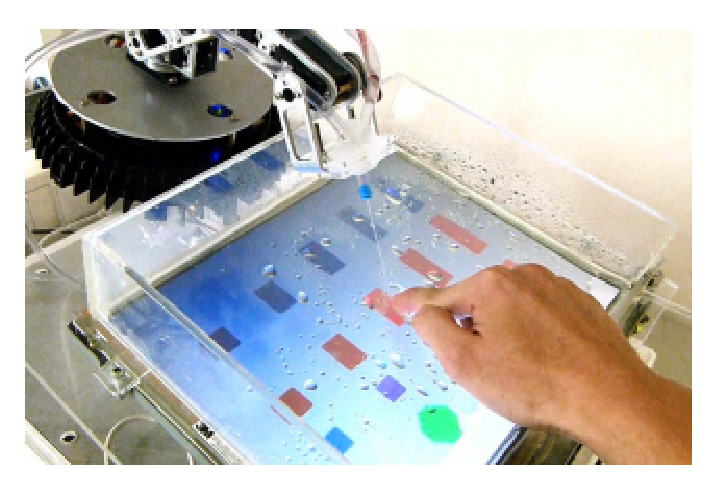
\includegraphics[width=8cm]{fig/figure6.eps}
  \caption{水流による触覚フィードバックシステムLiquiTouch}
  \end{center}
\end{figure}


%5
\section{今後の予定}
%研究会とかHCIIとか書いておけば良いかと

\bibliographystyle{jalpha}
\bibliography{shokunyu}
\end{document}
